\chapter{Introduction}

\section{The Growing Threat of Wildfires}

In recent decades, a significant rise in the frequency of wildfires has been observed, as well as in the annual total area burned~\cite{Weber/WildfireTrends}.
A disturbing trend of increased occurrence of mega-fires (wildfires which burn more than \SI{400}{\km\squared}) is also noticed.
Figure~\ref{fig:west-usa-area-burned} shows that the annual total area burned in the western United States in the past seven decades is best approximated by an exponential growth curve, which is rather alarming.

\begin{figure}[tb]
    \centering
    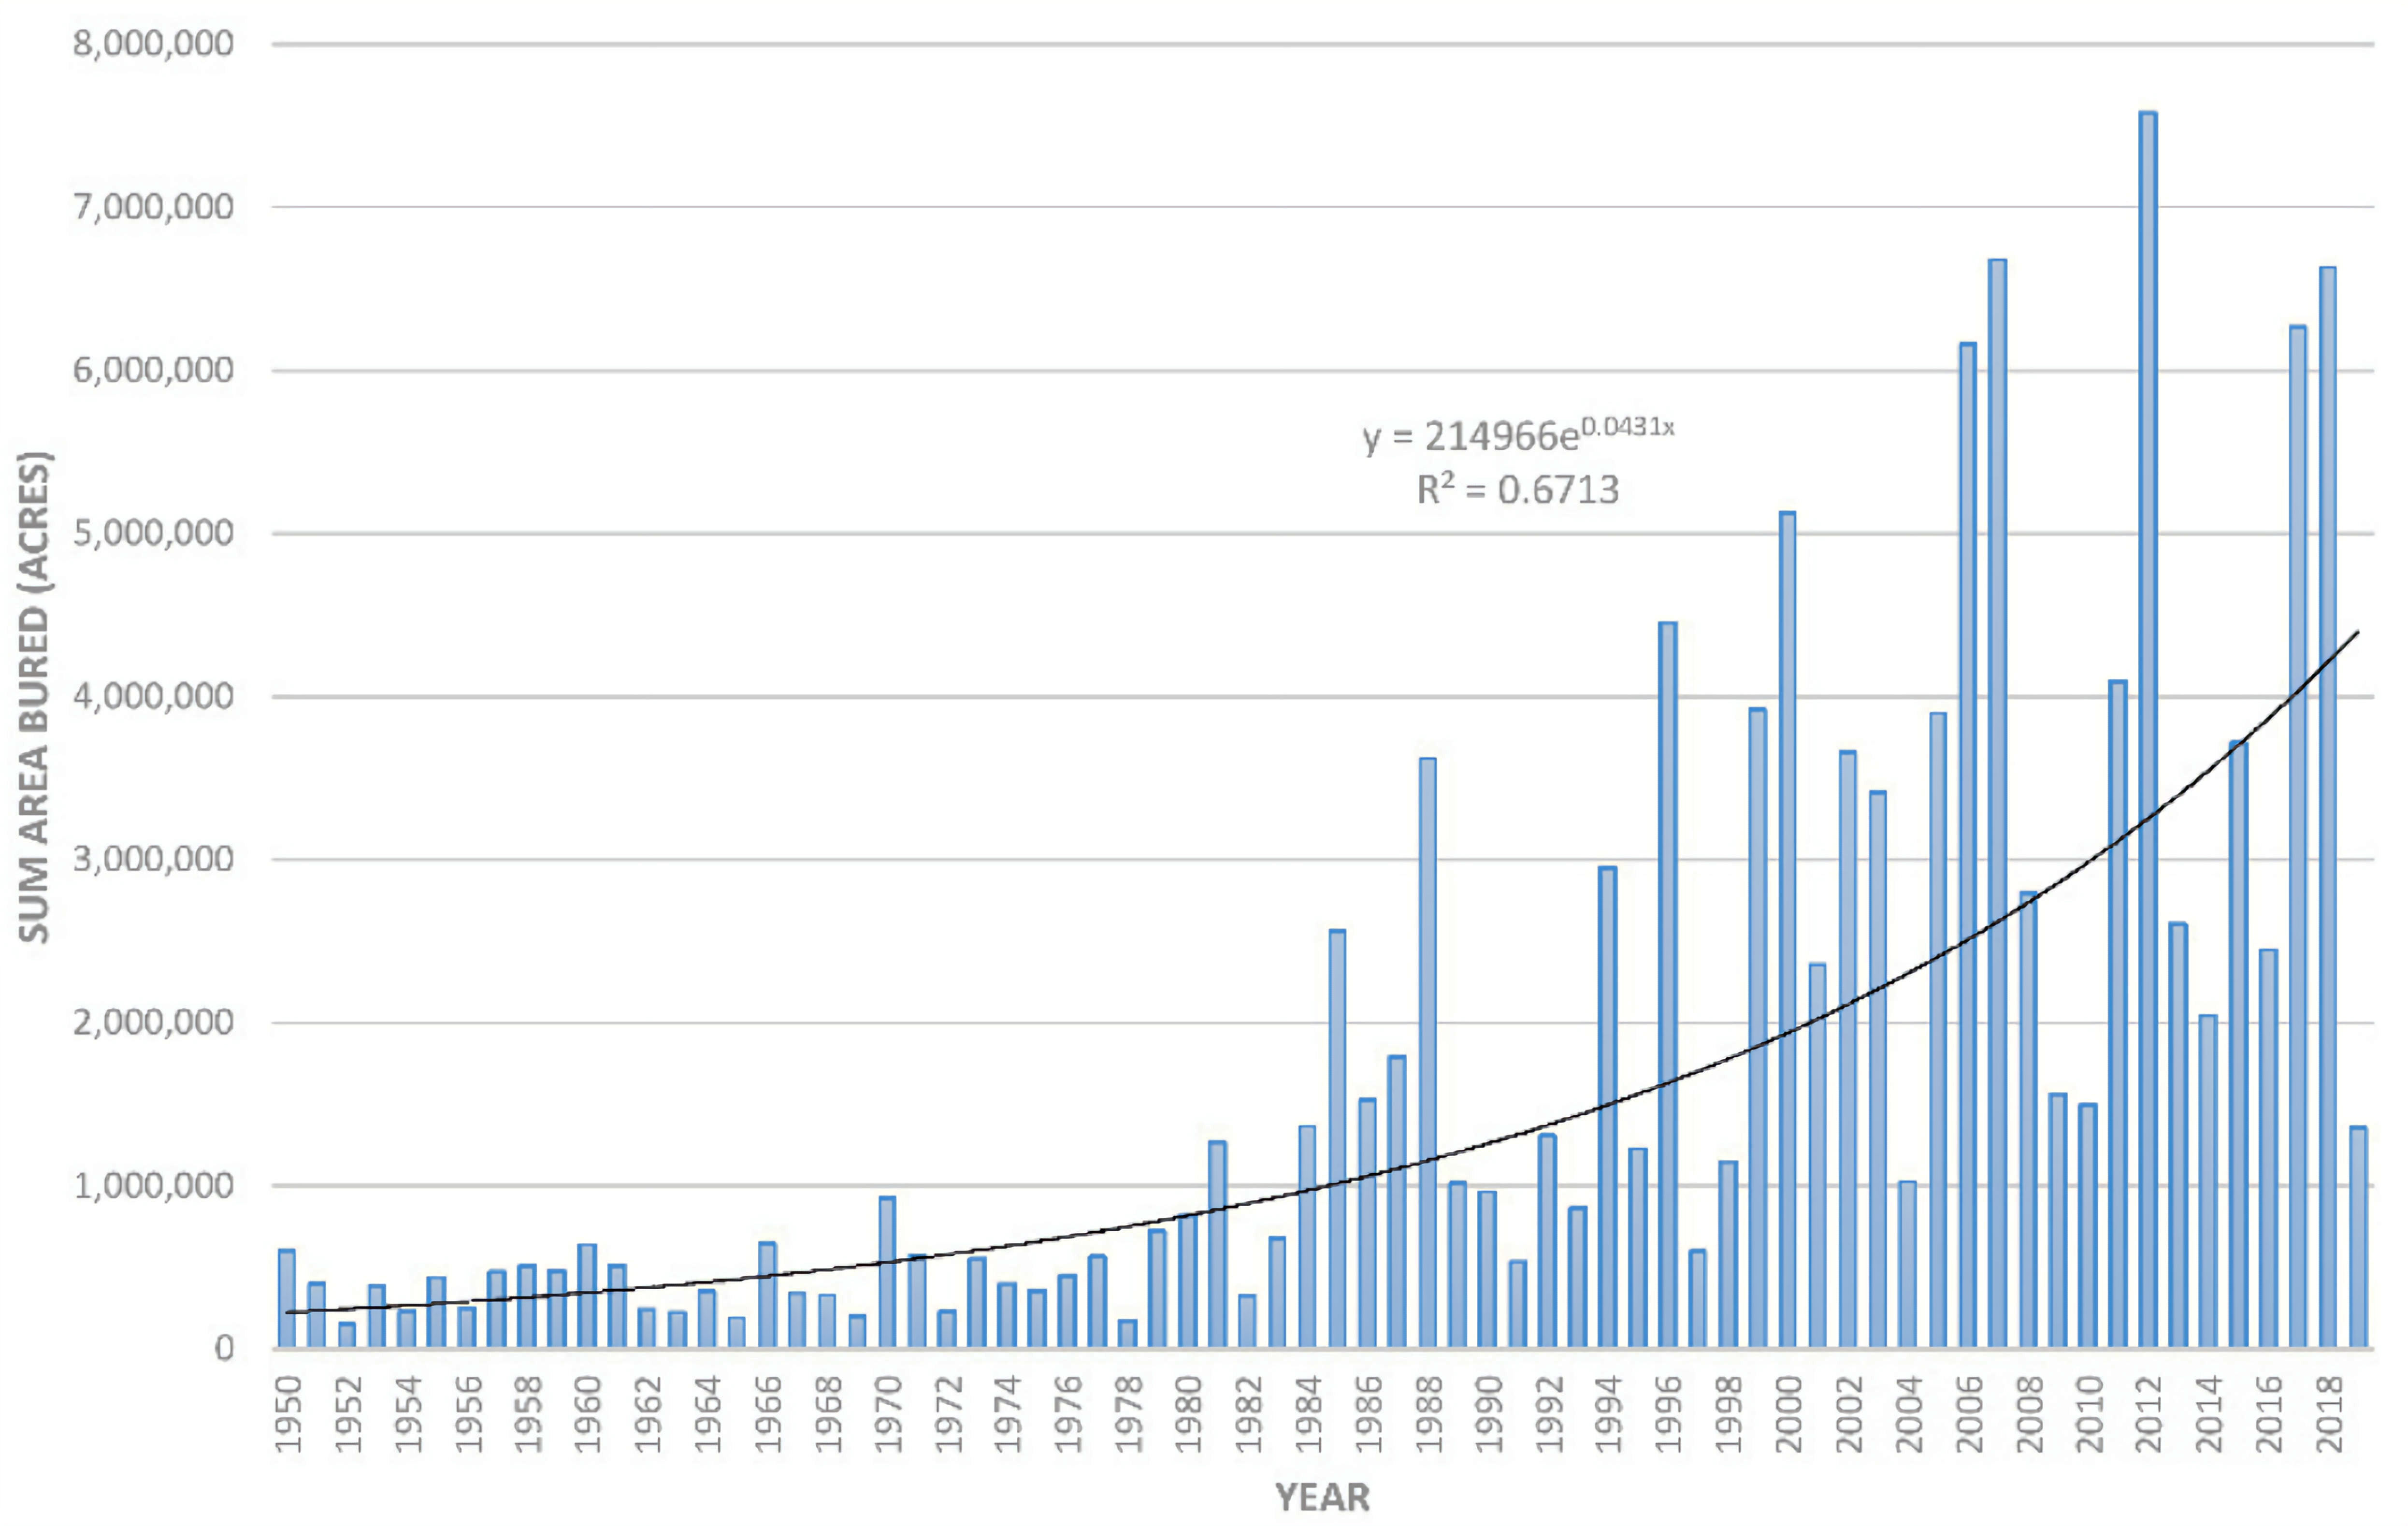
\includegraphics[width=0.9\linewidth]{img/west-usa-area-burned.jpg}
    \caption{The annual total area burned in western United States between 1950 and 2019~\cite{Weber/WildfireTrends}}
    \label{fig:west-usa-area-burned}
\end{figure}

The United Nations call for a radical change in how governments react to wildfires~\cite{UN/FiresReport}.
It is projected that climate change, as well as land-use change, will result in even more frequent and intense wildfires.
By 2050, a global increase in the likelihood of extreme wildfire events of up to $30\%$ can be expected, and even up to $50\%$ by the turn of the century.
Increased drought, high air temperatures, and low humidity, all of which are at least partially caused by the climate change, are classified as dangerous fire weather.
For example, nineteen of the hottest years since 1880 have occurred between the year 2000 and 2022~\cite{NASA/Temperature}.
Such weather is the cause of longer fire seasons, which in turn change the biomass and release more climate-changing carbon and other greenhouse gasses into the atmosphere, resulting in a positive feedback loop.

Spain faces similar difficulties as the rest of the world.
In 2021, the campaign to fight forest fires lasted from the middle of June until the end of October, coinciding with the period of the highest risk of wildfires.
A total of 73 aerial resources were available during the summer campaign~\cite{Spain/Campaign}.
A map of locations of preliminary amphibious airplane deployments for this campaign is shown in Figure~\ref{fig:spain-airplanes-deployment}.
On average, Spain faced approximately 11\,600 wildfires each year in the last decade.
One of the worst wildfires in its history occurred in September of 2021 in the province of Málaga, burning a total of approximately 8\,000 hectares of land.
On the 13th of September, 51 airplanes and helicopters were engaged in aerial firefighting to assist almost a thousand firefighters on the ground~\cite{ElMundo/Malaga}.

\begin{figure}[tb]
    \centering
    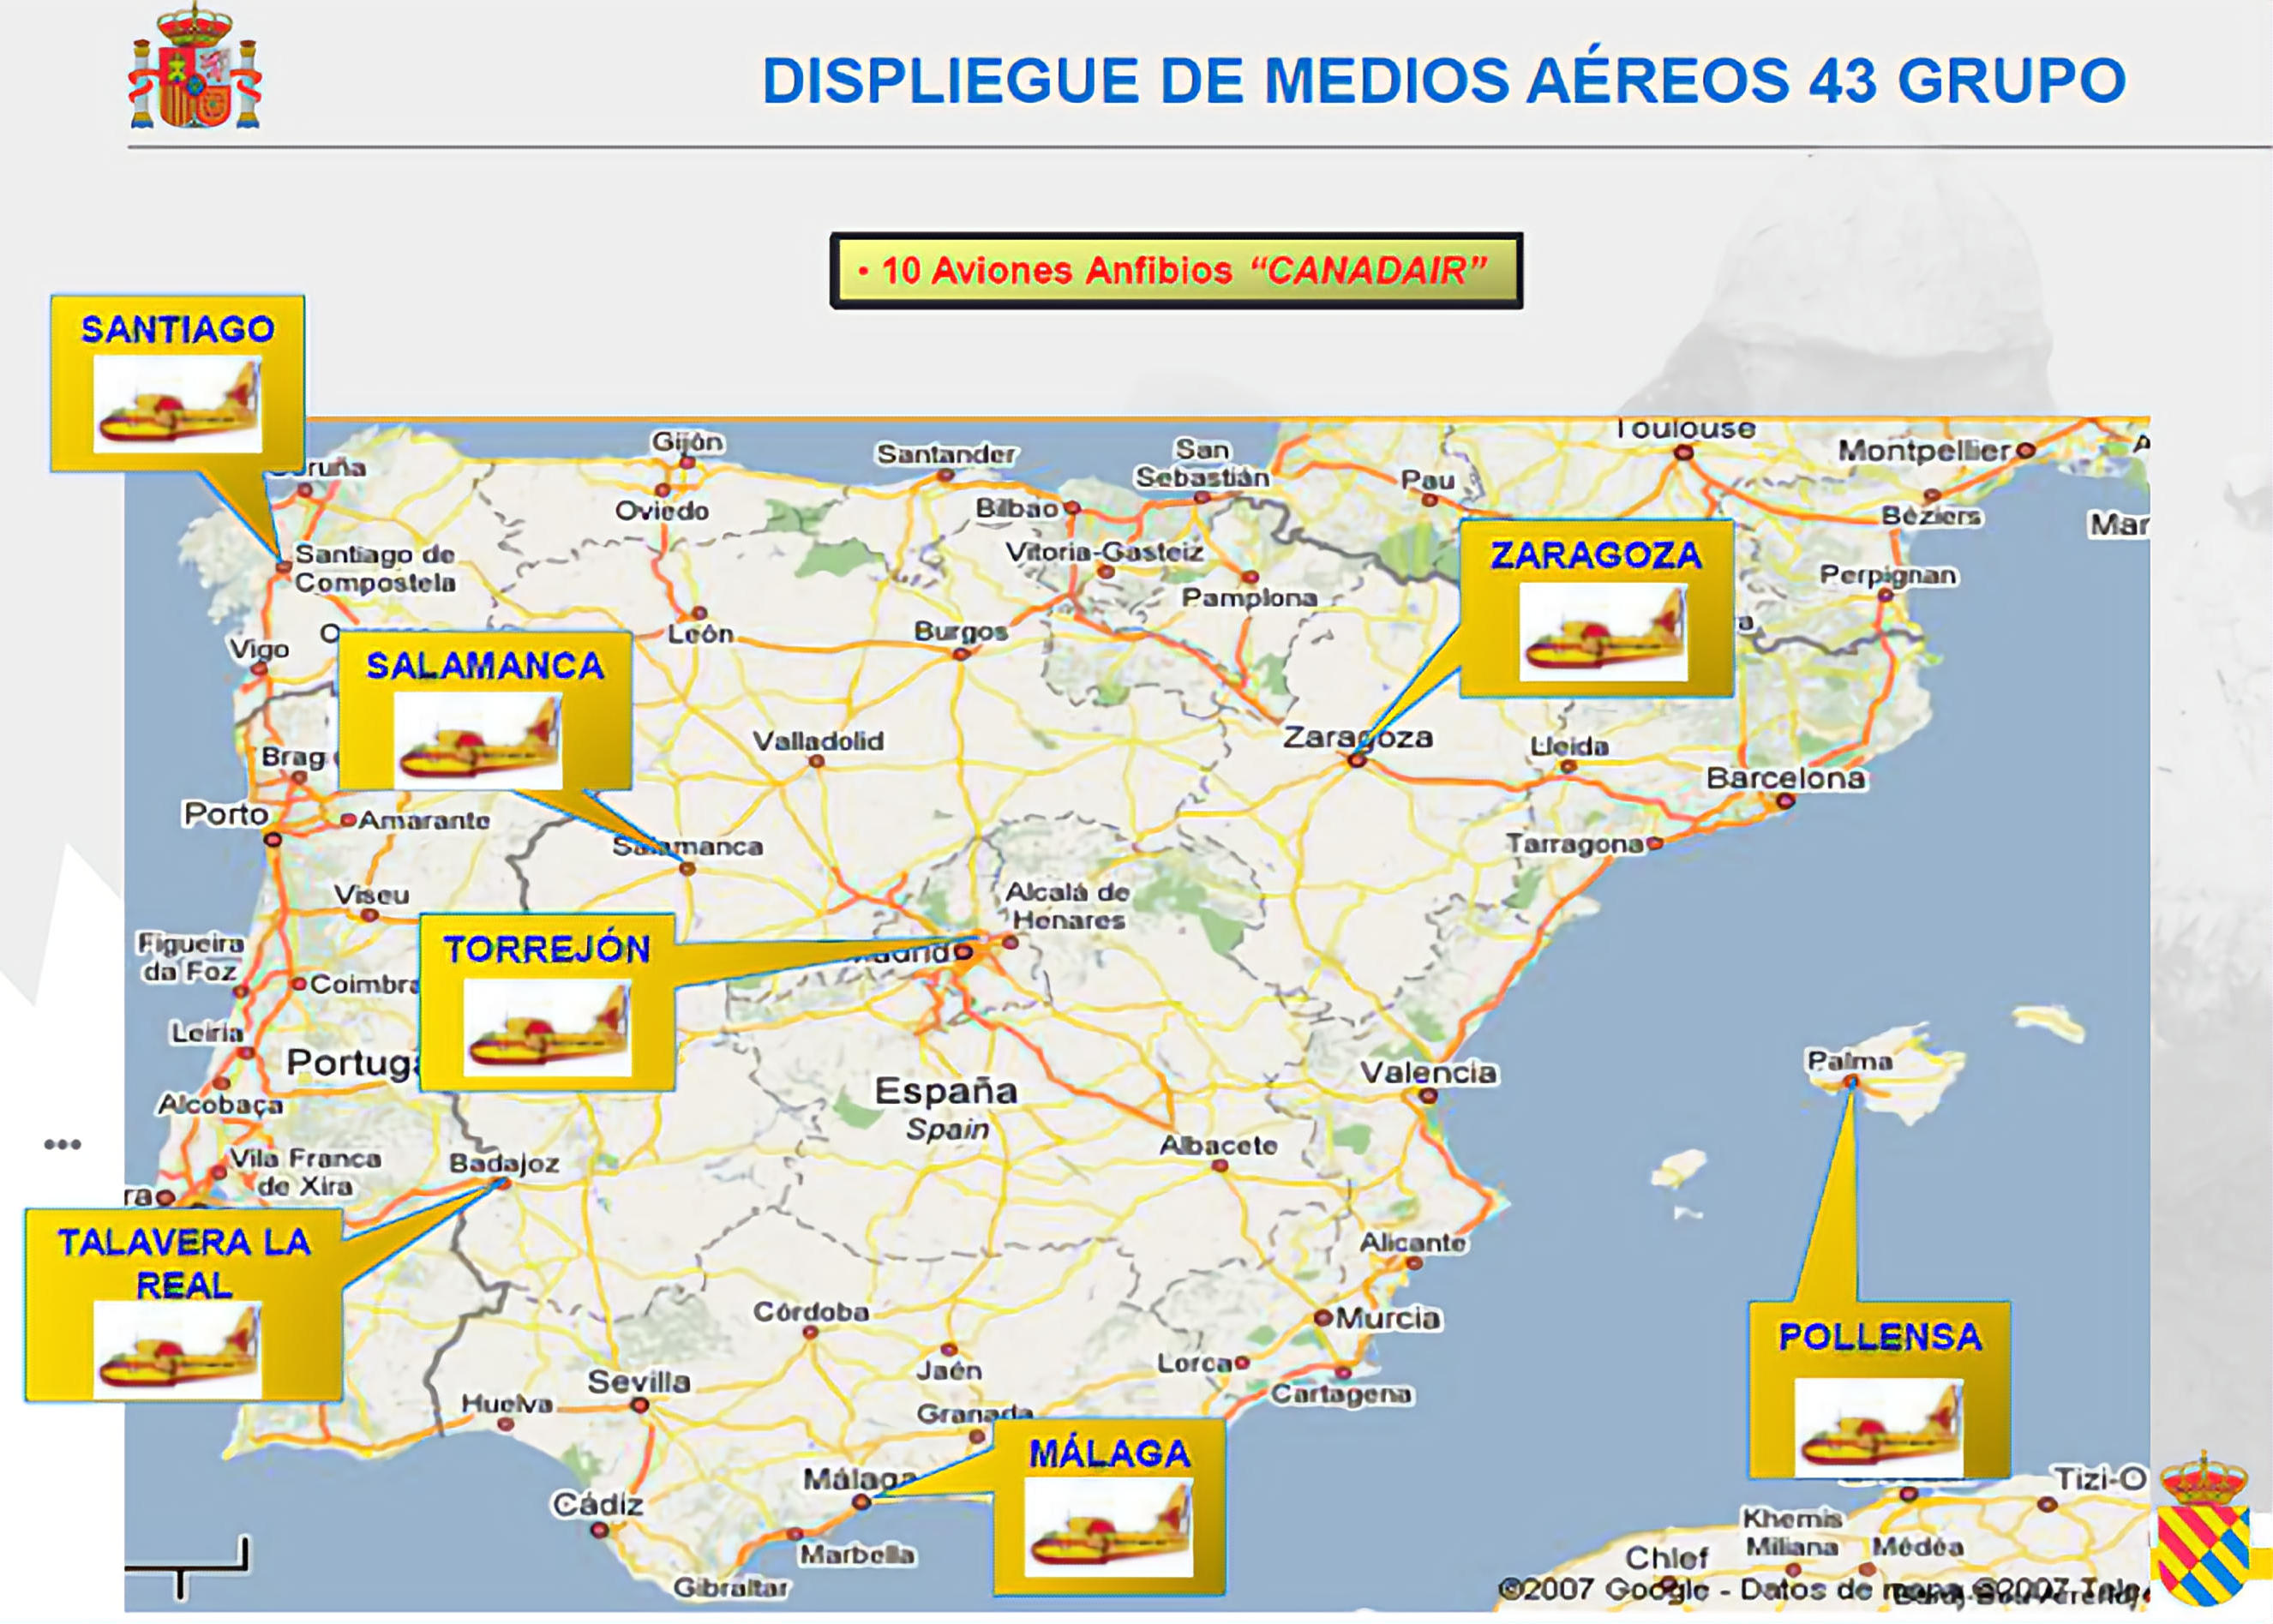
\includegraphics[width=0.9\linewidth]{img/spain-airplanes-deployment.jpg}
    \caption{A map of seaplane deployments in Spain in summer 2021~\cite{Spain/Campaign}}
    \label{fig:spain-airplanes-deployment}
\end{figure}


\section{Aerial Firefighting}

In order to extinguish or control a fire, either fuel, heat, or oxygen must be removed.
Aerial resources are frequently employed to combat wildfires by removing oxygen and heat, in a process called aerial firefighting.
They do not directly extinguish the fire, though, but support the firefighting crews on the ground in their suppression efforts~\cite{Canada/Suppression}.
Airplanes and helicopters drop water or chemical fire retardants near the edge of the burning fire, lowering the air temperature and sometimes creating a barrier between the wildfire and available fuels (firebreak)~\cite{Canada/Retardants}.\footnote{For simplicity, in this paper the term \textit{water} also implies \textit{fire retardants}, \textit{foam}, or any other chemical dropped by aerial resources.}
This allows for ground crews to come closer to the fire and put it out, or improve the created firebreak by removing the fuel (vegetation or other combustible material) with hand tools.

Wildfires of smaller scale are typically tackled in a prompt manner, with dynamic resource scheduling.
On the other hand, large-scale fires require complex protocols and planning models in order to use the available resources to their full potential, shortening the duration of the fire and minimizing the damage to the environment.
Large-scale wildfires typically have more than 20 active aerial resources and can last multiple days, or even weeks.
With such a high number of resources which must be efficiently scheduled arises a need for scalable algorithmic solutions.

This thesis explores a fast heuristic approach for scheduling resources employed in aerial firefighting, along with their assignment to individual areas of the fire, referred to as fire fronts.
The focus is put on extinction of large-scale forest fires, lasting several days.
The model and implementation cater to Spanish regulation of civil aviation~\cite{Spain/AnnexCircular}.
However, with minor changes depending on regulation and other specific requirements, it can be tailored to be applicable for use in other countries.


\section{Performance Goals}

The intended use of the implemented solution is in the planning phase for the next day.
Since aerial firefighting is only performed during the daylight hours, in summer months planning for the following day tends to take place approximately from 22:00 to 24:00.
This allows for a two hour time window in which the implemented algorithm has to find a satisfying solution.
Realistically, it is quite unlikely that the implementation will be run for longer than one hour.
In addition, it is preferable to have a faster variant which could be executed early in the morning in order to improve or modify the found solution in case parameters change (e.g., changes in weather conditions, changes in aircraft or pilot availability, etc.).
The faster variant might also need to be executed during the day for similar reasons.
Ideally, executing the faster variant should not take more than fifteen minutes.

Given these time constraints, it has been decided that, in the scope of this thesis, only one solution will be developed, with a target execution time of under 10 minutes, completely eliminating the need for a second, faster version.
Of course, the exact hardware used to execute the program will have a significant impact on real-world performance, especially if the algorithm benefits from parallelization.
For the purpose of this work, we make the conservative assumption that a mid-range processor (CPU) with four cores will be used, with a moderate amount of system memory (RAM).
That would be the equivalent of an average modern-day laptop.
Moreover, the size of a problem instance has a considerable influence on the time needed to solve it.
We tested the algorithm with a time limit of 10 minutes for large instances of 35 resources and five fire fronts.


\section{Thesis Structure}

This thesis is divided into nine chapters.
The second chapter gives an overview of related literature and existing solutions.
In the third chapter the problem and the model are defined in detail.
The fourth chapter proposes and explains the heuristic algorithm used to solve the problem, and provides the pseudocode.
The fifth chapter focuses on the implementation of the heuristic algorithm in software and elaborates on the formats of input and output data.
The sixth chapter describes which test scenarios were used to evaluate the implementation, and how they were generated.
In the seventh chapter the results are presented and compared with the solutions achieved by integer linear programming.
The eighth chapter proposes changes which could be made in order to improve the quality of the solutions.
The ninth chapter contains the final remarks.
The thesis ends with a list of references, three appendices containing examples of input and output files, and an abstract.
